\section{Deep models detail}
\label{sec:Deep models detail}
% 7 pages
The research of deep learning is a hot topic in contemporary computer science fields, and the design ideas between different deep models are also mutually influential.
% The transformer model gradually replaced the recurrent neural network (RRN) with sequential computing restriction and long-term memory loss issues.
% Innovative design concepts from the transformer model are also carried forward in the fields of computer vision.
% Many recent studies, such as Data-efficient image Transformers (DeiT) and Shifted window (Swin) transformers, have improved widely-adopted CNN-only models such as VGG and ResNet by introducing the self-attention structures to achieve better performance.
\subsection{Convolutional neural network}
\citet{fukushima1980neocognitron}

\citet{zhang1988shift}

\begin{figure}[ht!]
    \centering
    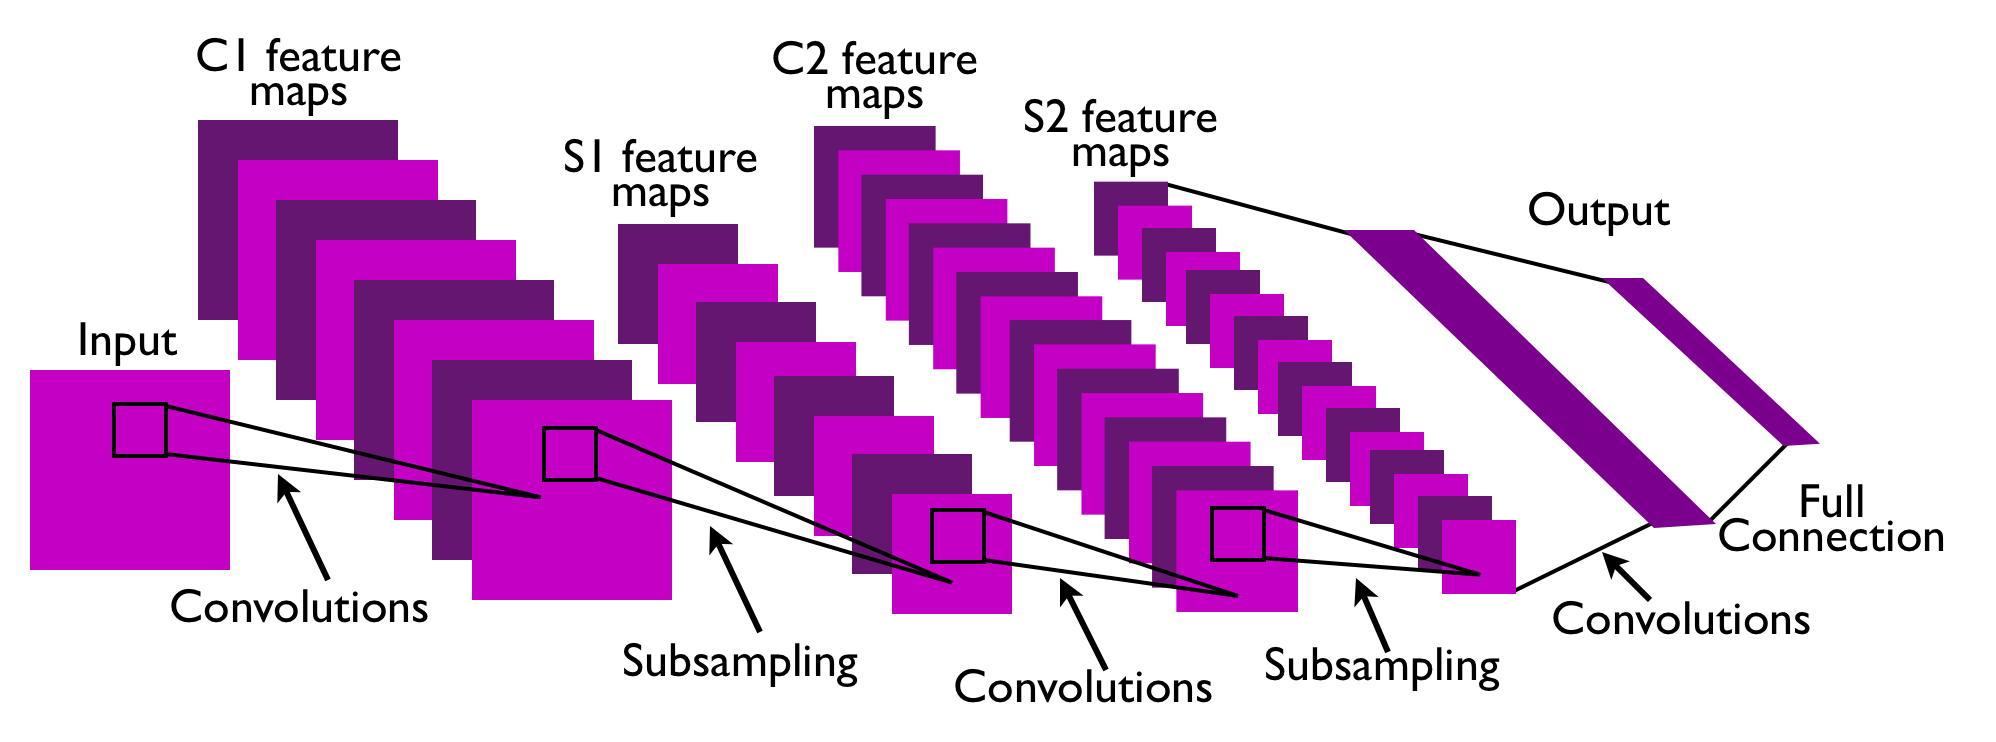
\includegraphics[width=\textwidth]{literature/imgs/ext-lecun-cnn-arch.png}
    \caption{CNN applications in vision by \citet{lecun2010convolutional}}
    \label{fig:ext-lecun-cnn-arch}
\end{figure}

\citet{lecun2010convolutional}

\citet{gu2018recent}

\subsection{Recurrent neural network}
\citet{jordan1997serial}

%LSTM
\citet{hochreiter1997long}

% RNN & LSTM fundamentals summary
\citet{sherstinsky2020fundamentals}

%GRU
\citet{chung2014empirical}

% et optimus
\subsection{Attention and Transformer}
%Attention
\citet{bahdanau2016neural}

\begin{minipage}[ht]{.6\textwidth}
    \begin{figure}[H]
        \centering
        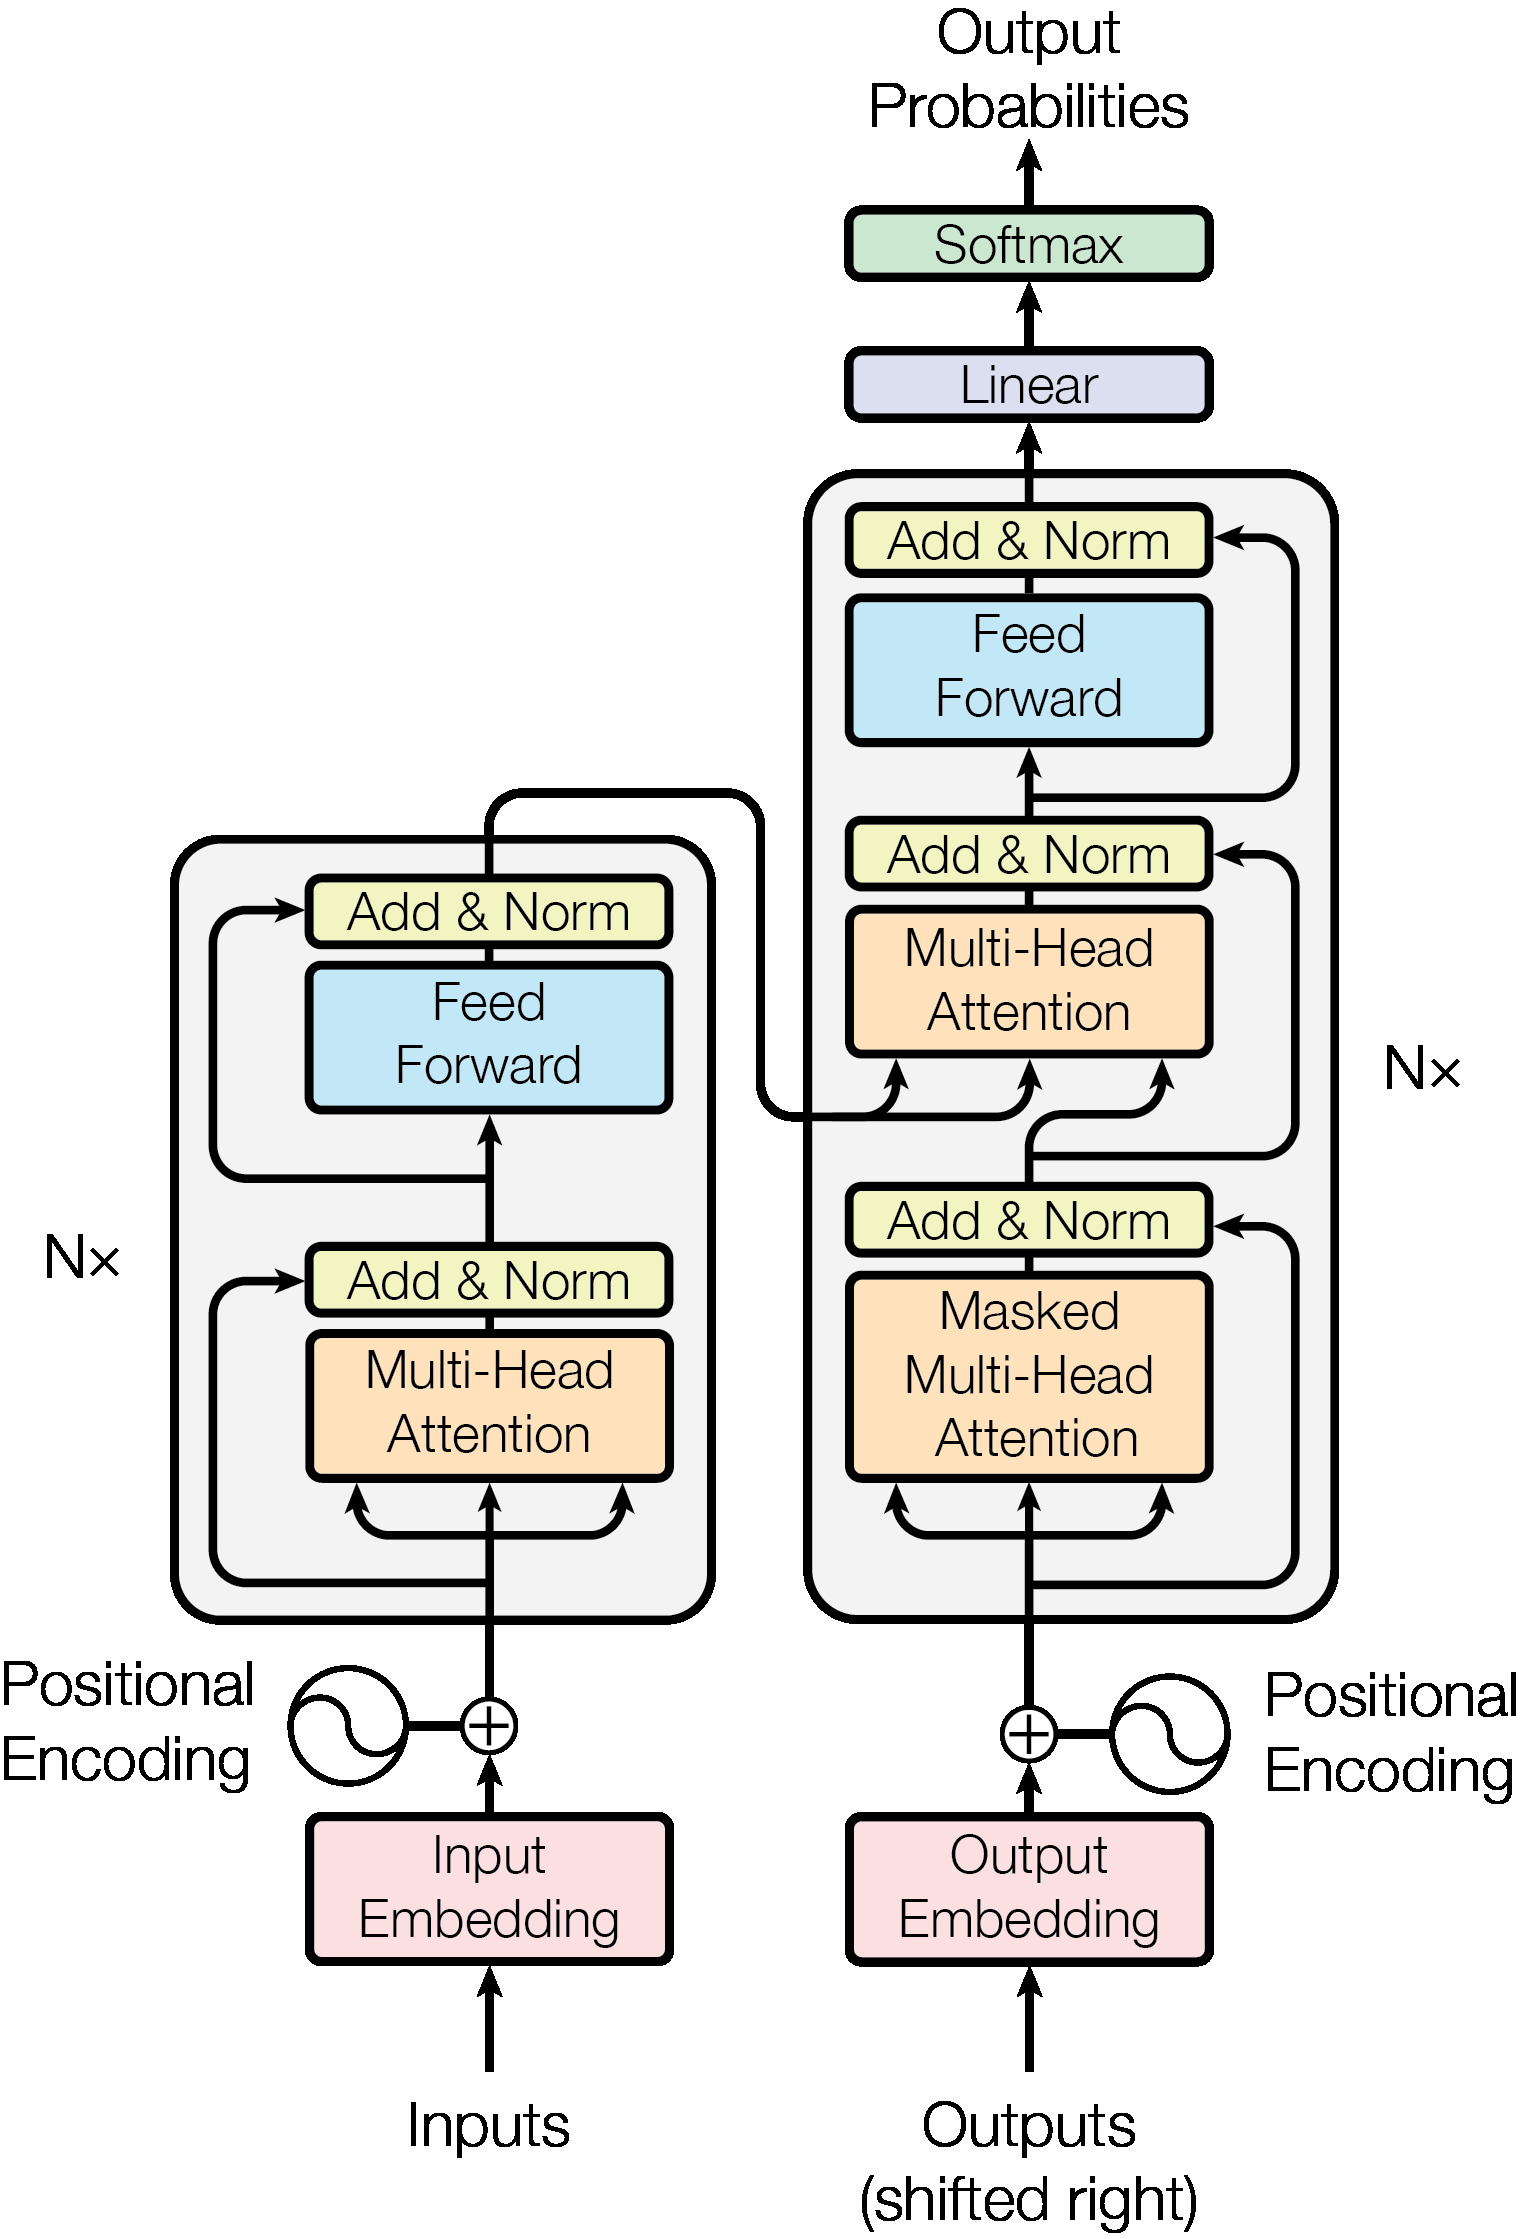
\includegraphics[width=\textwidth]{literature/imgs/ext-transformer.png}
        \caption{The Transformer model architecture \cite{vaswani2017attention}}
        \label{fig:ext-transformer}
    \end{figure}
\end{minipage}
\begin{minipage}[ht]{.35\textwidth}
    \centering
    \begin{figure}[H]
        \centering
        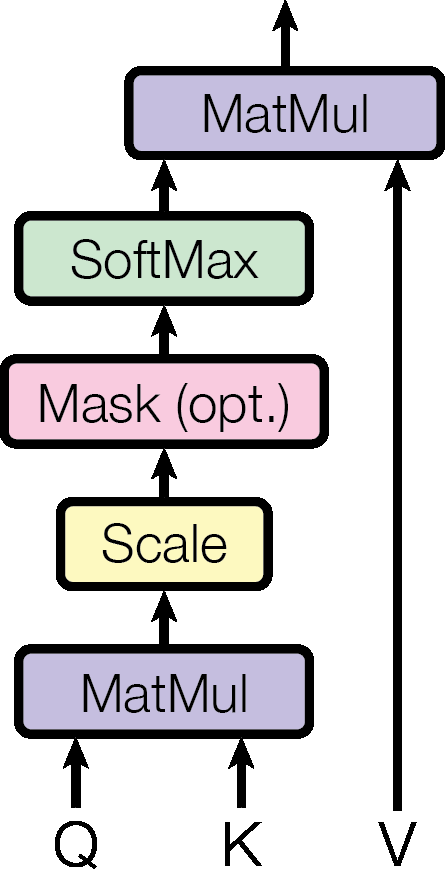
\includegraphics[width=.48\textwidth]{literature/imgs/ext-attention-dot-product.png}
        \caption{Scaled Dot-Product Attention \cite{vaswani2017attention}}
        \label{fig:ext-attention-dot-product}
    \end{figure}
    \vspace*{-.5cm}
    \begin{figure}[H]
        \centering
        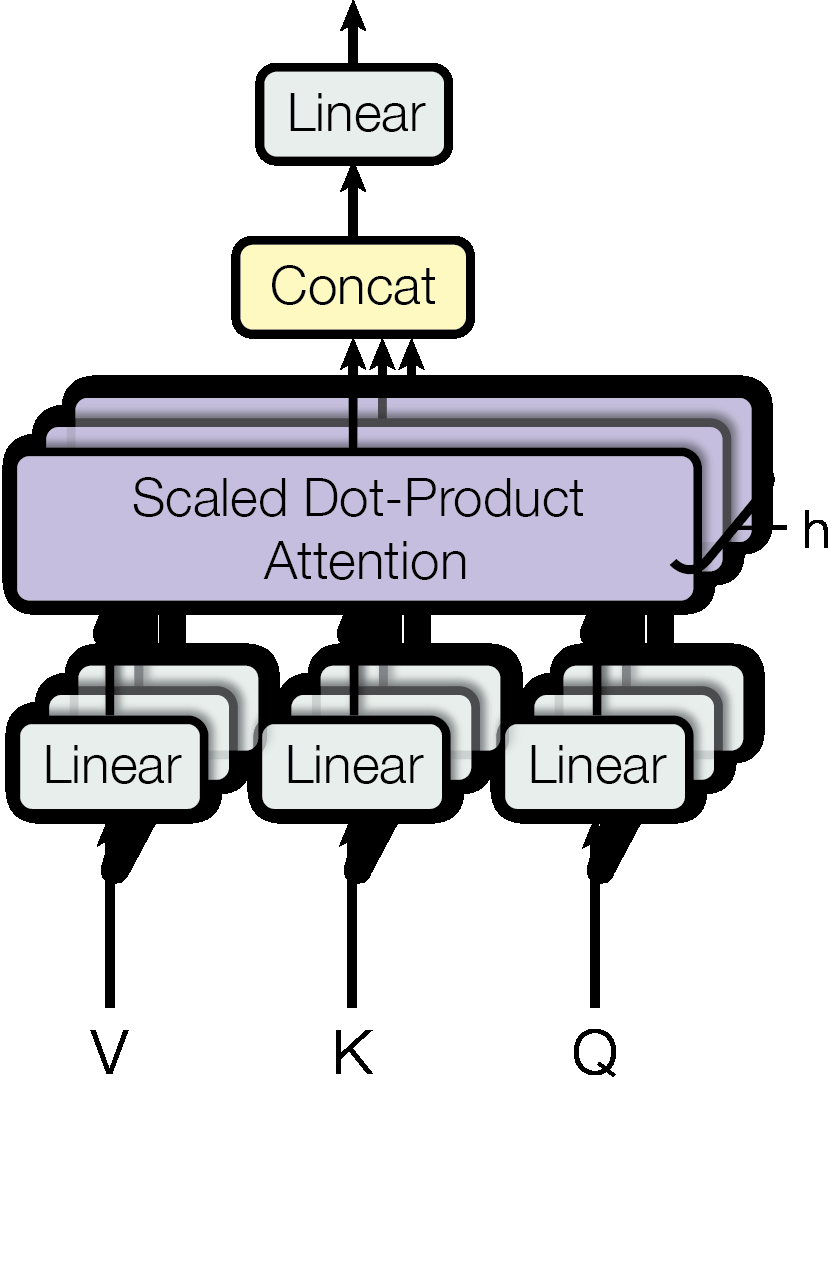
\includegraphics[width=.9\textwidth]{literature/imgs/ext-attention-multihead.png}
        \vspace*{-.4cm}
        \caption{Multi-Head Attention \cite{vaswani2017attention}}
        \label{fig:ext-attention-multihead}
    \end{figure}
\end{minipage}

\citet{vaswani2017attention}

%Transformer
While convolutional neural network (CNN) is in the ascendant among the fields of computer vision, transformer model composed of self-attention structures has achieved state-of-the-art results in many natural language processing tasks.

\citet{devlin2019bert}

% \citet{lohit2019temporal}

\subsection{State-of-the-art models}

\citet{srinivas2021bottleneck}

\citet{wang2021pyramid}

\citet{dai2021coatnet}
